% TODO: remove
\newpage

\section{Coulomb-Nuclear Interference}
\label{sec:coulomb}

\> outline for this section

\> reason for using 90m data
\> different ways of using 1000 and 90m data: combined (democratically), combined (each DS used where strong)

%----------------------------------------------------------------------------------------------------

\subsection{Theoretical Framework}
\label{sec:cni framework}

In this section the different components of the combined elastic scattering cross-section, already briefly outlined in the introduction, are discussed in more detail. In particular, the Coulomb amplitude (Section~\ref{sec:cni coulomb}), the nuclear amplitude (Section~\ref{sec:cni nuclear}) and their interference (Section~\ref{sec:cni interference}).

%------------------------------------------------------------------
\subsubsection{Coulomb Amplitude}
\label{sec:cni coulomb}
%
The Coulomb amplitude can be calculated from QED (e.g.~Section 3.2 in \cite{block06}), using empirical electric ${\cal F}_{\rm E}$ and magnetic ${\cal F}_{\rm M}$ form factors of the proton. It can be shown (e.g.~Section 1.3.1 in~\cite{jan_thesis}) that, at low $|t|$, the effect of both form factors can be described by a single function ${\cal F}$:
\begin{equation}
\label{eq:coul cs}
	{\d\sigma^{\rm C}\over \d t} = {4\pi\alpha^2\over t^2}\,{\cal F}^4\ ,\ 
	{\cal F}^2 = {{\cal F}_{\rm E}^2 + \tau {\cal F}_{\rm M}^2\over 1 + \tau}\ ,\ 
	\tau = {|t|\over 4m^2}\ ,
\end{equation}
where $\alpha$ denotes the fine-structure constant and $m$ represents proton mass.

The form factors by Pucket et al.~\cite{puckett10} are used in this study and it will be shown that different choices have negligible impact on results presented later on.


%------------------------------------------------------------------
\subsubsection{Nuclear Amplitude}
\label{sec:cni nuclear}

From first principles, very little conclusions can be made on the nuclear amplitude. Instead, several phenomenology or theory motivated descriptions will summarised here. The choice will be critically discussed later in Section~\ref{sec:cni task discussion}.

%--------------------
\vskip3mm
\hbox to\hsize{\bf Modulus\hfil}

At $|t| \gtrsim 0.02\un{GeV^2}$ the effects due to the Coulomb interaction are not expected to be large (see Figure~\ref{fig:cni effect}). Thus, the measured cross-section can be -- to large extent -- attributed to the nuclear component. Following Table~\ref{tab:data} and especially \cite{8tev-90m} which presents high-precision data for $|t| < 0.2\un{GeV^2}$, it is reasonable to parametrise the nuclear modulus as
\begin{equation}
\label{eq:nuc mod}
\left | {\cal A}^{\rm N}(t) \right | = a \exp\left( \sum\limits_{n = 1}^{N_b} b_n\, t^n \right)\ ,
\end{equation}
where $N_b$ gives the number of free parameters in the exponent. This parametrisation is also compatible with a number of theoretical models (see e.g.~\cite{elegent}).

Since the calculation of Coulomb-nuclear interference may, in principle, involve integrations (e.g.~Eq.~(\ref{eq:int kl})), it is necessary to extend the parametrisation meaningfully to $|t| > 0.2\un{GeV^2}$. Therefore, at $|t| > 0.05\un{GeV^2}$, the parametrisation is anchored to a preliminary cross-section from the same data set as in \cite{8tev-90m} which features a very similar dip-bump structure as at $\sqrt{s} = 7\un{TeV}$ \cite{epl95}. The region $0.2 < |t| > 0.5\un{GeV^2}$ is reserved for a smooth transition between the parametrisation in Eq.~(\ref{eq:nuc mod}) and the anchored part. It will be shown that changing the high-$|t|$ part has negligible impact on the results presented later on.


%--------------------
\vskip3mm
\hbox to\hsize{\bf Phase\hfil}

% ***
A {\it constant phase} is obviously the simplest choice:
\begin{equation}
\label{eq:nuc phase con}
\arg {\cal A}^{\rm N}(t) = p_0 = \hbox{const.}
\end{equation}
Note that this is equivalent to a strict proportionality of real and imaginary part of the amplitude at all $t$.

% ***
The {\it standard phase} parametrisation,
\begin{equation}
\label{eqn:nuc phase std}
\arg {\cal A}^{\rm N}(t) = p_{0} + \arctan \left(\frac{|t|-|t_{0}|}{\tau}\right) -  \arctan \left(\frac{-|t_{0}|}{\tau}\right) \: ,
\end{equation}
implements the main features of many theoretical models -- almost imaginary amplitude in the forward direction ($p_0 \approx \pi/2$) while almost purely real in the (first) diffraction dip. The parameters $t_0 = - 0.50\un{GeV^2}$ and $\tau = 0.1\un{GeV^2}$ have been chosen such that the shape is similar to a number of model predictions, see Figure~\ref{fig:phase illustration}.

% ***
Another parametrisation is by {\em Bailly et al.}~\cite{bailly87}:
\begin{equation}
\label{eq:nuc phase bai}
	%\arg {\cal A}^{\rm N}(t) = {\pi\over 2} - \arctan {\rho_0\over 1 - {t\over t_{\rm d}}},\ \rho_0 = {1\over \tan p_0}
	\arg {\cal A}^{\rm N}(t) = \arctan \left[ \tan p_0 \left(1 - {t\over t_{\rm d}} \right) \right]\ ,
\end{equation}
where $p_0$ determines the phase value at $t=0$ and $t_{\rm d} \approx -0.53\un{GeV^2}$ gives the position of the diffractive minimum at $8\un{TeV}$ (preliminary result from $90\un{m}$ data). This phase has behaviour qualitatively similar to the model of Jenskovszky et al., see Figure~\ref{fig:phase illustration}.

% ***
The {\it peripheral phase} \cite{kl94} provides an alternative to the above descriptions. Its parametrisation
\begin{equation}
\label{eq:nuc phase per}
\arg {\cal A}^{\rm N}(t) = p_0 - A \exp\left[ \kappa \left( \log {t\over t_{\rm m}} - {t\over t_{\rm m}} + 1 \right) \right]
\end{equation}
%results in a peak at $t_{\rm m} \approx -0.310\un{GeV^2}$, with amplitude $A \approx 5.53$ and width controlled by $\kappa \approx 4.01$.
results in a peak at $t = t_{\rm m}$, with an amplitude $A$ and width controlled by $\kappa$, as can be seen in Figure~\ref{fig:phase illustration}.

\begin{figure*}
\begin{center}
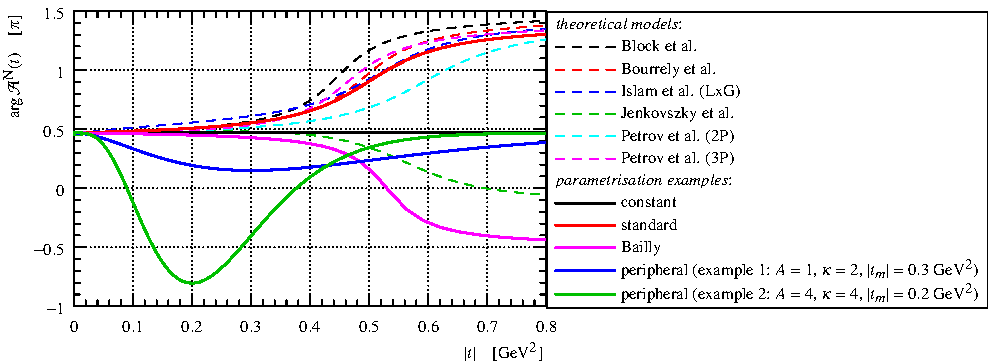
\includegraphics{fig/hadronic_phase_illustration.pdf}
\caption{Illustration of nuclear-phase forms. The dashed lines correspond to predictions by theoretical models (\cite{elegent} and references therein). The solid lines give typical examples of parametrisations used in the study, all at the same value of $\rho = 0.10$.
}
\label{fig:phase illustration}
\end{center}
\end{figure*}

Figure~\ref{fig:phase illustration} presents a comparison of phase predictions of several models to typical examples of parametrisations proposed above.

It should be noted that the phase has decisive influence on the amplitude behaviour in the space of impact parameter, $b$, see e.g.~Section 3 in~\cite{klk02}. It can be quantified by evaluating the root-mean-squares (RMS) of $b$ for elastic and inelastic collisions. The constant, standard and Bailly phases lead to elastic collisions more central (smaller RMS) than the inelastic ones. The peripheral phase can yield a description with the opposite hierarchy, which is argued more natural by some authors (e.g. Section~4 in~\cite{kl96}).

%------------------------------------------------------------------
\subsubsection{Coulomb-Nuclear Interference Formulae}
\label{sec:cni interference}

The {\bf simplified West-Yennie formula (SWY)} \cite{wy68} is derived in the framework of perturbative QFT by evaluating the lowest-order Feynman diagrams that comprise both nuclear and Coulomb interactions. In this approach, the interference is reduced to an additional phase between the Coulomb and nuclear amplitudes. Moreover, several approximations were used in the derivation. First, in order to avoid integrating over off-mass-shell contributions to the nuclear amplitude (purely known), very slow variation of the nuclear amplitude phase was assumed: $\arg {\cal A}^{\rm N} \approx \hbox{const}$. Then, in order to obtain a closed-form expression, the exponential slope of the nuclear modulus
\begin{equation}
\label{eq:nuc slope}
B^{\rm N}(t) = {\d \log |{\cal A}^{\rm N}|^2 \over \d t}
\end{equation}
was assumed constant (i.e.~$b_2 = b_3 = 0$ in parametrisation Eq.~(\ref{eq:nuc mod})). The original formula did not contain the electromagnetic form factor ${\cal F}$, it was added later by hand:
\begin{equation}
\label{eq:int swy}
	\begin{aligned}
		{\d\sigma\over \d t}^{\rm C+N} &= {\pi (\hbar c)^2 \over s p^2} \left | {\alpha s\over t} {\cal F}^2 \e^{\I\alpha \Phi(t)} + {\cal A}^{\rm N} \right |^2\ ,\cr
		\Phi(t) &= - \left( \log {B^{\rm N} |t|\over 2} + \gamma \right)\ ,\cr
	\end{aligned}
\end{equation}
where $\alpha$ is the fine structure constant and $\gamma \doteq 0.577$ the Euler constant. Despite the many limitations, the formula has extensively been used in past data analyses. For backward-comparison reasons we consider it also in this report.

The {\bf Kundr\' at-Lokaj\' i\v cek formula (KL)} \cite{kl94} was derived in an impact parameter formalism and it is based on the additivity of eikonals. The derivation poses no limitations on nuclear amplitude and the formula naturally incorporates the electromagnetic form-factor. In this treatment, the interference effect goes beyond a single phase, the $\Psi$ quantity is complex, in general:
\begin{equation}
\label{eq:int kl}
	\begin{aligned}
		{\d\sigma\over \d t}^{\rm C+N} &= {\pi (\hbar c)^2 \over s p^2} \left | {\alpha s\over t} {\cal F}^2 + {\cal A}^{\rm N} \e^{\I\alpha \Psi(t)} \right |^2\ ,\cr
		\Psi(t) &= 
			- \int \d t'\, \log {t'\over t} {\d\phantom{t'}\over \d t'} {\cal F}^2(t') \cr
		&\phantom{=} + \int \d t' \left( {{\cal A}^{\rm N}(t') \over {\cal A}^{\rm N}(t)} - 1 \right) { I(t, t')\over 2\pi }
			\ ,\cr
		I(t, t') &= \int_0^{2\pi} \d\phi\ {{\cal F}^2(t'')\over t''}\ , \cr
		t'' &= t + t' + 2\sqrt{t\, t'} \cos\phi\ ,\cr
	\end{aligned}
\end{equation}
where the $t$ integrations go over the entire kinematically allowed region.

For the calculations presented later on the Elegent implementation \cite{elegent} of the formulae will be used, together with the form-factor of Puckett et al.~\cite{puckett10}.

By analysing the formulae Eq.~(\ref{eq:int swy}) and (\ref{eq:int kl}), one can conclude that in the region where the nuclear amplitude dominates ($|t| \gtrsim 0.003\un{GeV^2}$), the effects due to the Coulomb interaction can be proportional either to $\alpha$ or to the ratio ${\cal A}^{\rm C} / {\cal A}^{\rm N}$. In both cases, the magnitude of the interference effects can be expected at a percent level, as shown in Figure~\ref{fig:cni effect}. The figure also shows that the effects at different $|t|$ probe different parts of the nuclear phase: maximum sensitivity to $\rho$ lies at very low $|t|$ while at higher $|t|$ the effects are sensitive to phase values at higher $|t|$. Another observation that one make from the figure is that for constant and standard phase (and can be generalised to Bailly, too) the effects are very similar, rather mild at higher $|t|$. This can be understood from a very limited variation of the phase at low $|t|$, which is the region contributing most to the integral in Eq.~(\ref{eq:int kl}). In contrary, the higher $|t|$ response to peripheral phases can have various forms, often similar to the ``U shape'' of the reconstructed cross-section, see Figures \ref{fig:fits common con} and \ref{fig:fits common per}.



\begin{figure*}
\begin{center}
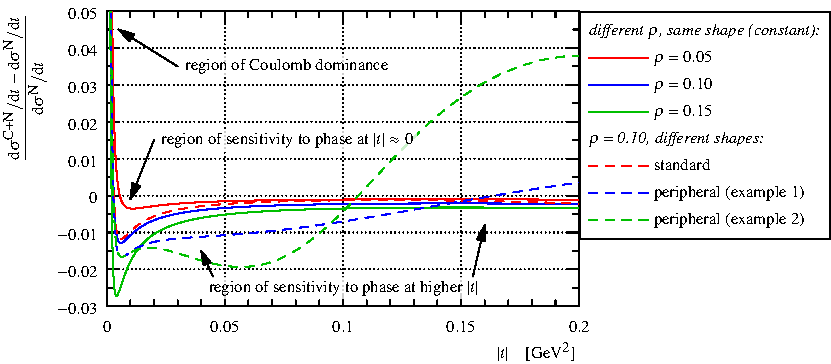
\includegraphics{fig/cni_effect_illustration.pdf}
\caption{%
Illustration of the effects due to the Coulomb interaction, using KL formula. For SWY formula, the picture is similar, however it misses the effects at higher $|t|$. The curves show a response of the interference formula to different nuclear phases with a purely exponential nuclear modulus. The solid curves correspond to phases of the same shape (constant) but different values of $\rho$ (maximal response can be seen at $|t| \lesssim 0.01\un{GeV^2}$). Conversely, the dashed lines correspond to phases with fixed $\rho$ but various shapes (the same examples as in Figure~\ref{fig:phase illustration}), with response sizeable at $|t| \gtrsim 0.02\un{GeV^2}$.
}
\label{fig:cni effect}
\end{center}
\end{figure*}

%----------------------------------------------------------------------------------------------------
\subsection{Fitting and parameter inference}
\label{sec:cni fitting}

%------------------------------------------------------------------
\subsubsection{Task analysis / general discussion ??}
\label{sec:cni task discussion}

As formalised in Section~\ref{sec:cni interference}, the observable cross-section can be split into two components: nuclear (as in the limit $\alpha\to 0$) and CNI (Coulomb effects as shown in Figure~\ref{fig:cni effect}).

As a next task it would be desirable to exploit the measured data to make statements about the nuclear component (e.g.~determine $a$ related to the total cross-section, see Eq.~(\ref{eq:si tot})) and the CNI component (e.g.~determine $\rho$). For this, it is essential to be able to separate the two cross-section components, which in turn requires them to be sufficiently distinct. Failing that, would lead to a situation characterised by degeneracy, many possible data descriptions and thus non unique statements about the two components.

The task is technically achieved by fitting. Therefore one needs to introduce parametrisations for the variable description elements: nuclear modulus and phase. Here it is important to realise that the form of the parametrisations defines what features can possibly be observed in the nuclear and CNI components of the cross-section. Therefore, the parametrisations define the level of distinction between the two components. For example, giving too much flexibility to the parametrisations will necessarily make the nuclear and CNI cross-section components undistinguishable and lead to degeneracy in the fit results. This tends to be the case with the peripheral phase parametrisation, Eq.~(\ref{eq:nuc phase per}), and large $N_b$ in the nuclear modulus parametrisation, Eq.~(\ref{eq:nuc mod}). These considerations illustrate that the choice of the parametrisations is crucial. At the same time, there is no rigorous guide for the choice which makes it subjective and arbitrary.

It is clear that not all possible nuclear modulus and phase parametrisations can be tested and therefore all results presented hereafter will have the character of examples. The choice of parametrisations in Section~\ref{sec:cni nuclear} is rather conservative and follows the guideline of minimal extensions with respect to previous TOTEM analyses \cite{8tev-90m}. It is easily conceivable to construct parametrisations that might yield few percent difference in parameters of interest, like $\rho$ or total cross-section. This applies mainly to the modulus parametrisation. Although at $|t| \gtrsim 0.02\un{GeV^2}$ the Coulomb effects are not large and thus the measured cross-section provides a good guide for parametrisations, at very low $|t|$ the measured data are dominated by the Coulomb interaction and no information on the nuclear component can be extracted. Consequently, the extrapolation to $t = 0$ is largely unconstrained. The uncertainty in nuclear phase might be less critical since the cross-section effects are limited by the KL/SWY interference formulae (see Figure~\ref{fig:cni effect}). This stems from the effects being predominantly sensitive to the nuclear phase at low $|t|$ and thus a large class of phase parametrisations could be reduced to a polynomial, by employing the Taylor expansion.

For the rest of the analysis, the following strategy has been adopted. Starting with the example parametrisations from Section~\ref{sec:cni nuclear}, the experimental data will be used to exclude the non-compatible ones. The rest will be used to present a matrix of conditional results, valid for one of the chosen parametrisation assumptions.



%------------------------------------------------------------------
\subsubsection{Fitting techniques}
\label{sec:cni fit techniques}

As already anticipated, it is vital to include the $\beta^* = 90\un{m}$ data to the fits. Formally, the data vector $\vec D$ can thus consist of rows of Table~\ref{tab:data} and/or Table~3 in \cite{8tev-90m}. The corresponding uncertainty matrix $\mat V$ includes two components. The statistical one contains the statistical uncertainties from the data tables on the diagonal. The systematic uncertainty component can be obtained from Eq.~(\ref{eq:covar mat}) and Eq.~(14) in \cite{8tev-90m}, assuming full correlation between the normalisation uncertainties in the two data sets (both calibrated to the same reference \cite{prl111}).


%-----------

Two alternative objective functions will be used for fitting in this report. The {\bf standard least squares (LS)} method suggests to minimise
\begin{equation}
\label{eq:chi sq LS}
	\chi_{\rm LS}^2 = (\vec D - \vec F)^\T\ \mat V^{-1}\ (\vec D - \vec F)\ ,
\end{equation}
where $\vec F$ is a vector of the fit function values at the data point abscissas (i.e.~at $t$ given by the ``representative point'' in the data tables).


%-----------

The {\bf parameter-comparison} method is based on decomposing both the data and fit function into a linear combination of features $\Phi_i(t)$:
\begin{equation}
\label{eq:parcmp decomposition}
	\vec D_j = \sum_i \zeta_i\ \Phi_i(t_j)\ ,\quad
	\vec F_j = \sum_i \eta_i\ \Phi_i(t_j)\ ,
\end{equation}
where $t_j$ represent the data point abscissas. The difference between the coefficients $\zeta_i$ and $\eta_i$ can then be used to establish the match quality between the data and the fit function. Such a test construction can offer several advantages. Since the estimation of coefficients $\zeta_i$ is likely to be binning-independent, so the test is (which is not the case of the standard LS approach). Another advantage comes from the possibility to choose the features $\Phi_i$: one can make separation between features expected in the data (e.g.~polynomials of low degree) from typical signatures of noise (e.g.~polynomials of high degree). This in turn leads to increased strength of the method. Regarding the technical implementation, a coordinate transformation is applied first:
\begin{equation}
\label{eq:parcmp transform}
	\vec D_i \rightarrow {\vec D_i - \vec F_i\over \vec F_i}\ ,
\end{equation}
which simplifies the task since the coefficients $\eta_i \equiv 0$ and also simplifies the choice of features $\Phi_i$. For these, polynomials of low degree have been chosen (cf.~data shape in Figure~\ref{fig:fits common con}) together with functions $1/t$ and $1/t^2$ relevant when fit functions do not describe the data well in the region of Coulomb dominance (see Figure~\ref{fig:cni effect}). For optimal performance, Gram-Schmidt orthonormalisation is applied such that $\Phi_i \cdot \Phi_j = \delta_{ij}$ which makes the determination of parameters straight-forward: \TODO{$\zeta_i = \Vec D \cdot \Phi_i$}. The scalar product has been chosen such that data points with larger uncertainties contribute less to the fit:
\begin{equation}
\label{eq:parcmp dot product}
	f \cdot g = \sum_{i, j} f(t_i)\ \mat V^{-1}_{ij}\ g(t_j) \ ,
\end{equation}
where $t_i$ are the abscissas of the data points and $\mat V$ is the data uncertainty matrix. This choice is also practical since the covariance matrix of the $\zeta_i$ parameters becomes a unit matrix: $\mat V_{\vec\zeta} = 1$. Moreover, the method becomes equivalent to the standard LS method in the limit where the number of features equals the number of data points. Finally, the fit quality is determined as a measure of compatibility of the vector $\vec\zeta$ with zero:
\begin{equation}
\label{eq:chi sq parcmp}
	\chi_{\rm PC}^2 = \vec\zeta^\T \mat V_{\vec\zeta}^{-1} \vec\zeta = |\vec\zeta|^2 \ .
\end{equation}
By Monte-Carlo simulations, it has been verified that the quantity $\chi_{\rm PC}$ has a chi-square distribution with the number of degrees of freedom (NDF) given by the number of features minus the number of free parameters. Because of that, fits with peripheral phase parametrisation will use more features ($t^0 \ldots t^8$) than fits with other phase parametrisations ($t^0 \ldots t^4$).

%-----------

Since both methods eventually rely on quantities with a chi-square distribution, the same fit quality measures can be quoted. The most straight-forward is the $\chi^2$ value after minimisation divided by NDF. A better statistical meaning has p-value, that is probability that a value at least as extreme as the observed one would be drawn from the corresponding chi-square distribution. The p-value can be conveniently expressed as significance which corresponds to a half-width of a central region that needs to be excluded from a normal distribution to give the same integrated probability as the p-value. The significance is given in multiples of $\sigma$, the standard deviation of the normal distribution.



%----------------------------------------------------------------------------------------------------
\subsection{Common fits of 1000 and 90m data}
\label{sec:cni common fits}

This section presents results for fits where the $1000$ and $90\un{m}$ data act in equal manner. Technically, the data vector $\vec D$ consists of two sub-columns, one from each data sets.

Figure \ref{fig:fits common con} shows the fit results for the constant nuclear phase. The free parameters include: $a$ and $b_n$ in Eq.~(\ref{eq:nuc mod}) and $p_0$ in Eq.~(\ref{eq:nuc phase con}). One can observe that the standard LS and parameter-comparison fits give very similar results (up to a small difference in normalisation). Therefore, only the parameter-comparison method will be presented in what follows (as it has better sensitivity in addition). Similarly, for $N_b = 1$ the fits with SWY and KL interference formulae are almost identical, thus only KL will be used later on. Still for $N_b = 1$, note the very bad fit quality: more than $7\un{\sigma}$ for the standard LS and almost $10\un{\sigma}$ for the parameter-comparison method. Consequently, one may conclude that the combination of purely exponential nuclear modulus and constant phase is excluded by the data. Moreover, since this is the only combination theoretically compatible with the SWY interference formula, the formula is excluded, too.

Furthermore, as it could be expected from Figure~\ref{fig:cni effect}, the fits with constant, standard and Bailly nuclear phases are nearly identical. Therefore, the constant phase will be used hereafter to represent this group.

%\> Figure \ref{fig:fits common con}
%\>> std LS and par cmp fits very similar (up to small difference in normalisation), can be generalised to all results hereafter
%\>> $N_b = 1$ fits with KL and SWY almost identical (also true in what follows, will use KL to represent both)
%\>> case $N_b = 1$ + constant phase excluded by both fit techniques
%\>>> the only compatible with SWY $\Rightarrow$ SWY excluded, too
%\>> addition (not shown): results for standard and Bailly phase (almost) indistinguishable from the constant one, will use only constant to represent this ``family''

\begin{figure*}
\begin{center}
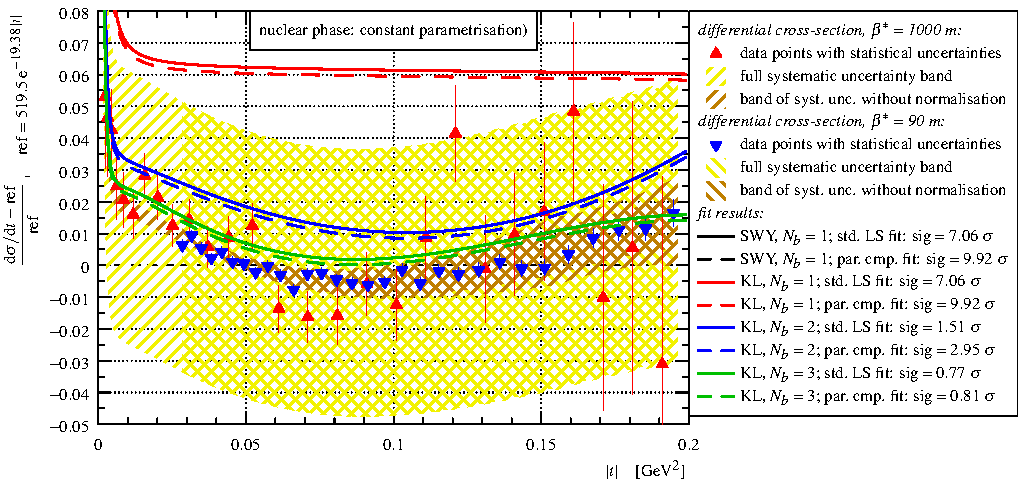
\includegraphics{fig/fits_common_con.pdf}
\caption{%
Fit results for fits with constant nuclear phase, Eq.~(\ref{eq:nuc phase con}). The vertical axis gives the cross-section difference from a reference exponential. The red (blue) triangles represent the $\beta^* = 1000$ ($90\un{m}$) data with their statistical uncertainties. The systematic uncertainties are represented by the hatched bands: yellow (full uncertainty), brown (all systematic uncertainties except for normalisation). The orientation of the hatching indicates the respective data set.
The curves represent fit results obtained with different parametrisations and fit techniques. The solid curves represent standard least-squares fits, the dashed ones fits with the parameter-comparison method. Different colours stand for different interference formulae (SWY/KL) and numbers of parameters in the nuclear modulus exponent, $N_b$, cf.~Eq.~(\ref{eq:nuc mod}). The red curves almost fully cover the black ones. The legend gives fit quality (significance) for each of the fits.
}
\label{fig:fits common con}
\end{center}
\end{figure*}

Figure \ref{fig:fits common per} shows the fit results for the constant nuclear phase. The free parameters include: $a$ and $b_n$ in Eq.~(\ref{eq:nuc mod}) and $p_0$, $A$, $\kappa$ and $t_m$ in Eq.~(\ref{eq:nuc phase per}). Again, one may conclude that the standard LS fits are very similar to those from the parameter-comparison method (up to a small difference in normalisation for $N_b = 1$). In contrast to the fits with constant nuclear phase, here all the fits have reasonable quality.

\begin{figure*}
\begin{center}
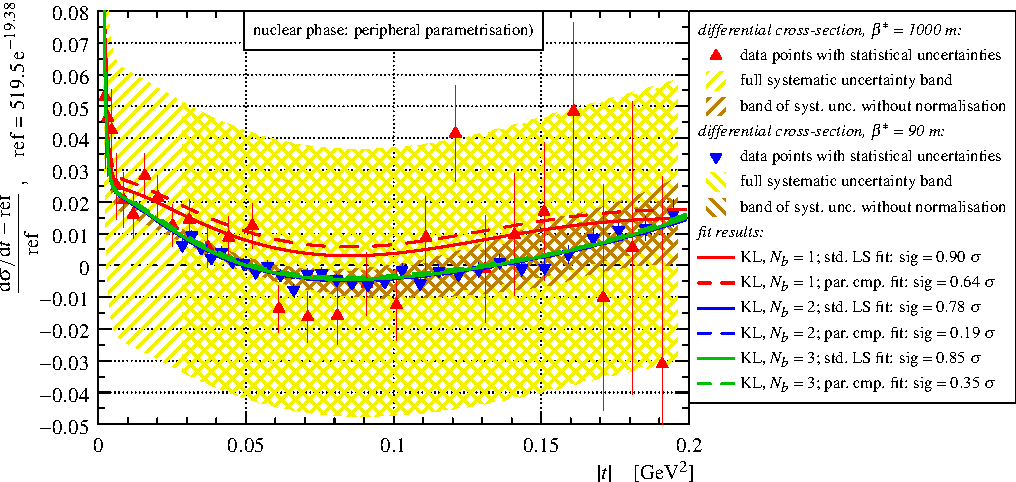
\includegraphics{fig/fits_common_per.pdf}
\caption{%
Fit results for fits with peripheral nuclear phase, Eq.~(\ref{eq:nuc phase per}). Legend identical as in Figure~\ref{fig:fits common con}. \TODO{repeat the legend if not on the same page}
}
\label{fig:fits common per}
\end{center}
\end{figure*}


From the fits presented in Figures~\ref{fig:fits common con} and \ref{fig:fits common per} one may derive parameters of interest related to the nuclear component. In particular $\rho = 1 / \tan p_0$, exponential slope $B^{\rm N}$, cf.~Eq.~(\ref{eq:nuc slope}), and the total cross-section via the optical theorem:
\begin{equation}
\label{eq:si tot}
\sigma_{\rm tot}^2 = {16\pi\, (\hbar c)^2\over 1 + \rho^2}\, \left. \d\sigma^{\rm N}\over\d t\right|_0
		= {16\pi^2\, (\hbar c)^4\over s p^2 (1+\rho^2)}\, a^2\ ,
\end{equation}
where $a$ is the intercept of the nuclear modulus parametrisation, cf.~Eq.~(\ref{eq:nuc mod}). The results are summarised in Table \ref{tab:fits common} and visualised in Figure~\ref{fig:fits reciprocal der} (black points).

There are several trends observable in the results. For the fits with constant phase, the values of $B^{\rm N}$ and $\rho$ increase with $N_b$. This can be understood from Figures~\ref{fig:cni effect} (constant phase cannot make any sizeable CNI effect at higher $|t|$) and \ref{fig:fits common con} (data have a ``U shape'' with respect to the reference exponential). Therefore, fits with $N_b = 1$ (looking almost as a straight line in the relative frame of Figure~\ref{fig:fits common con}) can only reflect a mean slope of the data, which is lower than a realistic one when extrapolated to $t = 0$. Consequently, adding more flexibility to the nuclear modulus ($N_b = 2, 3$) makes the fits absorb more of the ``U shape'' of the data and thus extrapolate to $t = 0$ with a higher value of the slope $B^{\rm N}$. A similar argumentation may applied to the trend of $\rho$ values. For positive values of $\rho$ the CNI effect leads to a negative interference (see Figure~\ref{fig:cni effect}) and thus $\rho$ can be deduced from the gap between data at low $|t|$ and the extrapolation from higher $|t|$ (where the strong constraint from the $90\un{m}$ data applies). Consequently, fits extrapolating to $t = 0$ too low yield also low values of $\rho$ (or even negative) and vice versa.

In the case of fits with peripheral phase, the trend is less clear which can be expected from Figure~\ref{fig:cni effect} since the CNI effects can absorb large part of the ``U shape''.

The total cross-section results are rather stable, with mild dependence on $N_b$ and phase choice (with a small exception of the combination of $N_b = 2$ with peripheral phase).

Figure~\ref{fig:fits reciprocal der} also compares the newly derived parameters to previous TOTEM measurements and other predictions. For the total cross-section, the new results occur consistently little higher than the value from \cite{prl111}. This is fully expectable since now the CNI effects (most importantly the negative interference due to $\rho$) are taken into account. The diffractive slope comparison to the result from \cite{prl111} is more delicate. In the present analysis, the results correspond to the slope of the nuclear component at $t = 0$. In the previous analysis, however, mean slope (over the range $|t| < 0.2\un{GeV^2}$) of combined (C+N) cross-section was evaluated. Moreover, the previous analysis did not include the optics matching procedure as the present one. The latter fact is responsible for the shift of central value (brown horizontal line) from the results for $N_b = 1$ and constant phase (left-most column). In principle, one would expect that this difference is covered by the yellow uncertainty band, however one should remember that in the previous analysis it only corresponds to the mean slope. And the uncertainty would increase if extrapolation to $t = 0$ is included.
%
Regarding $\rho$, the figure provides comparison to the preferred-model estimate by COMPETE \cite{compete} which is obtained by extrapolation from lower scattering energies. The new results lie all below the COMPETE value.

Monte-Carlo studies show that uncertainties of $\rho$ in Table~\ref{tab:fits common} have about equal source in statistical and systematic uncertainties of the data. For the slope $B^{\rm N}$, the uncertainty depends strongly of the fit configuration and the statistical and systematic uncertainties contribute at various fractions. The uncertainties of $\sigma_{\rm tot}$ are mostly due to the normalisation uncertainty.
\TODO{Check: from an old MC with 1000m data only!}

Table \ref{tab:fits common} gives also RMS values of impact parameter $b$ for elastic and inelastic collisions. These parameters quantify the character of the collisions in the impact parameter space and have been calculated according to Section 3 in~\cite{klk02} directly from $t$-space quantities. \TODO{equation??}
One can conclude that irrespectively on $N_b$, the constant-phase fits have central character: elastic collisions occur at smaller impact parameters than the inelastic collisions. In contrary, all the fits with the peripheral nuclear phase lead to opposite (peripheral) hierarchy.


\begin{table*}
\caption{%
Parameters derived from the parameter-comparison fits presented in Figures~\ref{fig:fits common con} and \ref{fig:fits common per}. The rows correspond to different numbers of parameters in the nuclear modulus exponent. The left-hand (right-hand) side columns refer to fits with constant, Eq.~(\ref{eq:nuc phase con}), (peripheral, Eq.~\ref{eq:nuc phase per}) nuclear phase. The RMS values of impact parameter $b$ correspond to elastic (el), inelastic (inel) and any (tot) collisions. The combination $N_b = 1$ with constant phase is set in gray as it is excluded by data, see Figure~\ref{fig:fits common con}.
}%
\vskip-3mm
\label{tab:fits common}
\begin{center}
\small
\setlength{\tabcolsep}{5pt}
%\def\arraystretch{0.8}
\begin{tabular}{c@{\hskip20pt}cc@{\hskip20pt}cc}
\hline
\hline
% header
	& \multispan2\hfil constant \hfil & \multispan2\hfil peripheral \hfil  \cr
\hline
 			& \color{gray}$\rho = -0.027 \pm 0.021$ & \color{gray}$\sqrt{\langle b^2\rangle_{\rm el}} = 0.87\un{fm}$					& $\rho = 0.083 \pm 0.023$ & $\sqrt{\langle b^2\rangle_{\rm el}} = 1.68\un{fm}$					\cr
$N_b = 1$	& \color{gray}$B = (19.39 \pm 0.05)\un{GeV^{-2}}$ & \color{gray}$\sqrt{\langle b^2\rangle_{\rm inel}} = 1.34\un{fm}$		& $B = (19.68 \pm 0.07)\un{GeV^{-2}}$ & $\sqrt{\langle b^2\rangle_{\rm inel}} = 1.03\un{fm}$		\cr
			& \color{gray}$\sigma_{\rm tot} = (103.8 \pm 2.1)\un{mb}$ & \color{gray}$\sqrt{\langle b^2\rangle_{\rm tot}} = 1.23\un{fm}$	& $\sigma_{\rm tot} = (102.8 \pm 2.1)\un{mb}$ & $\sqrt{\langle b^2\rangle_{\rm tot}} = 1.24\un{fm}$	\cr\hline
%                                                                                                                                                                                                                   
 			& $\rho = 0.059 \pm 0.021$ & $\sqrt{\langle b^2\rangle_{\rm el}} = 0.87\un{fm}$						& $\rho = 0.120 \pm 0.026$ & $\sqrt{\langle b^2\rangle_{\rm el}} = 1.90\un{fm}$						\cr
$N_b = 2$	& $B = (19.97 \pm 0.07)\un{GeV^{-2}}$ & $\sqrt{\langle b^2\rangle_{\rm inel}} = 1.36\un{fm}$		& $B = (20.46 \pm 0.44)\un{GeV^{-2}}$ & $\sqrt{\langle b^2\rangle_{\rm inel}} = 0.96\un{fm}$		\cr
			& $\sigma_{\rm tot} = (102.8 \pm 2.1)\un{mb}$ & $\sqrt{\langle b^2\rangle_{\rm tot}} = 1.25\un{fm}$	& $\sigma_{\rm tot} = (104.13 \pm 2.3)\un{mb}$ & $\sqrt{\langle b^2\rangle_{\rm tot}} = 1.28\un{fm}$	\cr\hline
%                                                                                                                                                                                                                   
 			& $\rho = 0.090 \pm 0.024$ & $\sqrt{\langle b^2\rangle_{\rm el}} = 0.87\un{fm}$						& $\rho = 0.115 \pm 0.026$ & $\sqrt{\langle b^2\rangle_{\rm el}} = 2.01\un{fm}$						\cr
$N_b = 3$	& $B = (20.39 \pm 0.14)\un{GeV^{-2}}$ & $\sqrt{\langle b^2\rangle_{\rm inel}} = 1.37\un{fm}$		& $B = (20.04 \pm 0.36)\un{GeV^{-2}}$ & $\sqrt{\langle b^2\rangle_{\rm inel}} = 0.82\un{fm}$		\cr
			& $\sigma_{\rm tot} = (102.5 \pm 2.1)\un{mb}$ & $\sqrt{\langle b^2\rangle_{\rm tot}} = 1.26\un{fm}$	& $\sigma_{\rm tot} = (103.5 \pm 2.2)\un{mb}$ & $\sqrt{\langle b^2\rangle_{\rm tot}} = 1.25\un{fm}$	\cr\hline
\hline
\end{tabular}
\end{center}
%\vskip-10mm
\end{table*}

The fits have been repeated with Borkowski electromagnetic form factors instead the default one (see Section~\ref{sec:cni coulomb}) leading to no change in the results. Similarly, another set of fits has been performed with the high-$|t|$ component of the nuclear modulus (see Section~\ref{sec:cni nuclear}) scaled by a factor of $1.2$ (preliminary uncertainty estimate), again with no impact on the results.



%----------------------------------------------------------------------------------------------------
\subsection{Reciprocally constrained 1000 and 90m fits}
\label{sec:cni reciprocal fits}

In contrast to the previous section, here the $1000$ and $90\un{m}$ data sets are assigned specific roles in the fit, naturally following from where each data set it strong. One can identify the following four elements of the fits.
\begin{itemize}
\item Modulus normalisation, parameter $a$ in Eq.~(\ref{eq:nuc mod}): both data set can be used equally well.
\item Modulus ``shape'', parameters $b_n$ in Eq.~(\ref{eq:nuc mod}): essential contribution from the $90\un{m}$ data set with very low statistical uncertainties.
\item Phase at $t = 0$, parameter $p_0$ in Eqs.~(\ref{eq:nuc phase con}) and (\ref{eq:nuc phase per}): as indicated in Figure~\ref{fig:cni effect}, maximum sensitivity to $p_0$ (or $\rho$) lies a $|t|$ region only available in the $1000\un{m}$ data set.
\item Phase ``shape'' (only for peripheral phase), other parameters in Eq.~(\ref{eq:nuc phase per}): as for modulus shape, the $90\un{m}$ data set provides much stronger constrains.
\end{itemize}
Therefore, one may perform a series of two fits, one with $1000$ and the other with $90\un{m}$ data set, each of them fixing the parameters according to the breakdown above. Since there are two choices for the modulus normalisation, $a$, and one can start the fit series with either the $1000$ or the $90\un{m}$ data set, there are four variants of this approach, see Figure~\ref{fig:fits reciprocal der}. Obviously, the fit series is repeated several times until convergence is reached.

Figure~\ref{fig:fits reciprocal der} presents a comparison of the fit results from methods proposed in this and the previous sections. For the fits with the peripheral phase, all phase parameters were free (as in the previous section). \TODO{describe observations}
\> generally, very similar results from all the fit methods (notable exceptions ??)
\> higher significance from 1000m data - why?
\> mainly for sigma tot: split to red-magenta and blue-green groups, according to which data set determines the normalisation

\begin{figure*}
\begin{center}
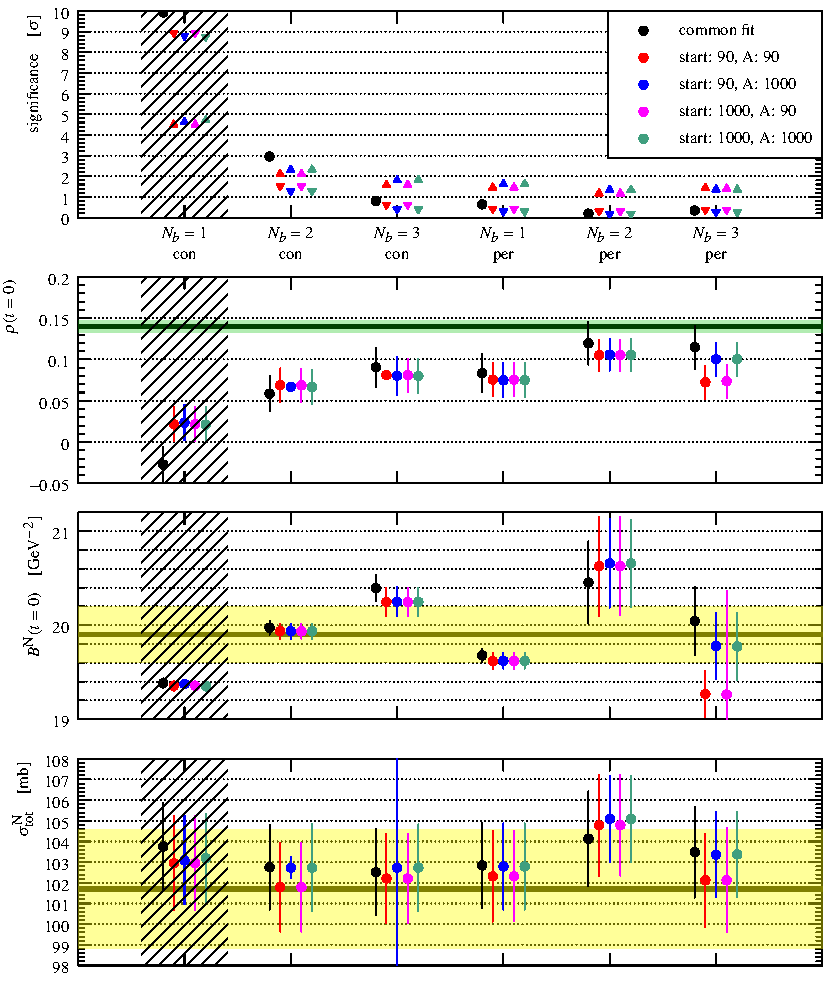
\includegraphics{fig/fits_reciprocal_derived.pdf}
\caption{%
Comparison of parameters derived from common fits (Section~\ref{sec:cni common fits}) and reciprocal fits (Section~\ref{sec:cni reciprocal fits}). The black points correspond to the results from Table~\ref{tab:fits common}. The other points represent the reciprocal fits as described in the legend. There ``start'' indicates the data set used first in the fit series and ``$a$'' indicates the data set determining the nuclear modulus normalisation (cf.~Eq.~(\ref{eq:nuc mod})). The significance plot gives fit quality for both fits in the series: triangles up (down) from $1000$ ($90\un{m}$) data set. The results are organised in 6 columns, each of them corresponds to a combination of $N_b$ and constant or peripheral phase. The left most column ($N_b = 1$ and constant phase) is hatched since this combination is excluded by data, note the very large significance. The yellow horizontal bands represent the previous measurements by TOTEM at the same energy \cite{prl111}. The green horizontal band stands for the preferred-model extrapolation of $\rho$ by COMPETE \cite{compete}.
\TODO{Reasonable error bars, point fluctuations}
}
\label{fig:fits reciprocal der}
\end{center}
\end{figure*}
